\documentclass[xcolor=dvipsnames]{beamer}
\makeatletter\def\Hy@xspace@end{}\makeatother 
\usepackage{graphicx, color, amssymb, amsmath, bm, rotating, graphics,
epsfig, multicol, amsthm}
\usepackage[english]{babel}
\usepackage[T1]{fontenc}
\usepackage[ansinew]{inputenc}
\usepackage[authoryear]{natbib}
%\newcommand{\newblock}{}  %needed to make beamer and natbib play nice
\usepackage{tikz}
%\usetheme{Boadilla}
%\usecolortheme{lily}
 \usecolortheme[named=Red]{structure}
% \setbeamercolor{structure}{bg=black}
% \setbeamercolor{structure}{fg=Goldenrod}
% \setbeamercolor{title}{bg=Black}
% \setbeamercolor{frametitle}{bg=Black, fg=Goldenrod}
% \setbeamercolor{title in head/foot}{fg=Black, bg=Goldenrod}
% \setbeamercolor{author in head/foot}{fg=Goldenrod, bg=Black}
% \setbeamercolor{institute in head/foot}{fg=Goldenrod, bg=Black}
% \setbeamercolor{date in head/foot}{fg=Goldenrod, bg=Black}
\setbeamercovered{transparent=0}
\beamertemplatenavigationsymbolsempty

\title[Stan for Spatial]{Introduction to Stan for Markov Chain Monte Carlo}

%\subtitle{}
\author[Matt Simpson]{Matthew Simpson}
\institute[Mizzou Statistics]{Department of Statistics, University of Missouri}

\begin{document}

\begin{frame}
\titlepage
\end{frame}

% \begin{frame}[fragile]
% \frametitle{Abstract}
% \centering
% In the first part of this talk I introduce Hamiltonian Monte Carlo (HMC) and its implementation in Stan. The focus is on building intuition and not on theory, e.g. for how HMC works, how Stan solves many of the problems typically associated with implementing HMC, and for why HMC and Stan are attractive alternatives to Gibbs based sampling algorithms. In the second part of the talk, I provide a brief introduction to using Stan with the \verb0rstan0 \verb0R0 package. I provide several examples in this portion of the talk, guidance for interpreting Stan's warning and error messages, and intuition for how to construct better HMC samplers using Stan.
% \end{frame}

\begin{frame}
\frametitle{Stan is...}

\begin{columns}[c]
 \begin{column}[c]{0.5\textwidth}

\begin{itemize}
\item[] 
\begin{center}
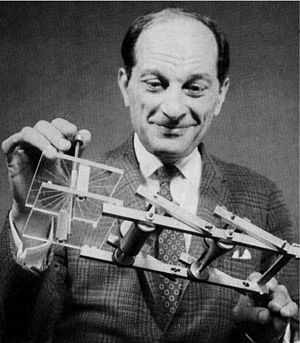
\includegraphics[width=0.5\textwidth]{stan.jpg}
\end{center}
\end{itemize}
\end{column}

\begin{column}[c]{0.5\textwidth}
\begin{itemize}
\item[] \textbf{Stanislaw Ulam}, inventor of Monte Carlo methods.\\
\end{itemize}
\end{column}
\end{columns}

\vspace{0.2cm}

\begin{itemize}
\item[] \url{http://mc-stan.org/}

\vspace{0.2cm}

\item[] A \textbf{probabilistic programming language} that implements {\color{red}\textbf{Hamiltonian Monte Carlo (HMC)}}, variational Bayes, and (penalized) maximum likelihood estimation.\\

\vspace{0.2cm}

\item[] Available on Linux, Mac, and Windows with interfaces in \textbf{R}, \textbf{Python}, shell (command line), MATLAB, Julia, Stata, and Mathematica.

\end{itemize}
\end{frame}

\begin{frame}
\frametitle{Markov chain Monte Carlo (MCMC)}
Goal: sample from some density $\pi(\bm{q})$.\\

\vspace{0.5cm}

Create a Markov chain with transition density $k(\bm{q}'|\bm{q})$.
\begin{itemize}
\item Start with arbitrary $\bm{q}^{(0)}$ and repeatedly sample $\bm{q}^{(t+1)} \sim k(\bm{q}'|\bm{q}^{(t)})$.\\

\vspace{0.2cm}

\item Under some conditions $\bm{q}^{(t)} \to \bm{q}$ in distribution.

\vspace{0.2cm}

\item Additionally with {\color{red}geometric ergodicity}:
\begin{align*}
  \frac{1}{T}\sum_{t=1}^T f(\bm{q}^{(t)}) \to \mathrm{N}\left(\mathrm{E}[f(\bm{q})], \frac{\mathrm{var}[f(\bm{q})]}{ESS}\right).
\end{align*}
\end{itemize}

\vspace{0.5cm}

Auxillary variable MCMC: construct a variable $\bm{p}$ with joint density $\pi(\bm{q},\bm{p}) = \pi(\bm{p}|\bm{q})\pi(\bm{q})$.
\begin{itemize}
\item Construct a Markov chain for $(\bm{q}, \bm{p})$ and throw away the sampled $\bm{p}^{(t)}$s.
\vspace{0.2cm}
\item Ex: data augmentation, slice sampling, HMC, etc.
\end{itemize}
\end{frame}

\begin{frame}
\frametitle{HMC in Theory}
Construct $\bm{p}$ in a special way. Let $\bm{q},\bm{p}\in \Re^n$ and:
\begin{itemize}
\item[] $V(\bm{q})\phantom{,\bm{p}} = -\log \pi(\bm{q})$ --- \emph{potential energy}.
\item[] $T(\bm{q}, \bm{p}) = - \log \pi(\bm{p} | \bm{q})$ --- \emph{kinetic energy}.
\item[] $H(\bm{q}, \bm{p}) = V(\bm{q}) + T(\bm{q}, \bm{p})$ --- \emph{Hamiltonian}, total energy. 
\end{itemize}
where $\bm{p}$ denotes \emph{position} and $\bm{q}$ denotes \emph{momentum}.

\vspace{0.3cm}

Energy-preserving evolution in time is defined by Hamilton's equations:
\begin{align*}
\frac{\mathrm{d}\bm{p}}{\mathrm{d} t} = - \frac{\partial H}{\partial \bm{q}}; && \frac{\mathrm{d}\bm{q}}{\mathrm{d} t} = + \frac{\partial H}{\partial \bm{p}}.
\end{align*}
How to implement HMC (in theory):
\begin{enumerate}
\item Sample $\bm{p}' \sim \pi(\bm{p}|\bm{q}^{(t)})$.
\item Run Hamiltonian evolution forward in time from $(\bm{q}^{(t)}, \bm{p}')$ for a some amount of \emph{integration time} to obtain $(\bm{q}^{(t+1)}, \bm{p}^{(t+1)})$.
\end{enumerate}
\end{frame}

\begin{frame}
\frametitle{HMC in Pictures}
\begin{center}
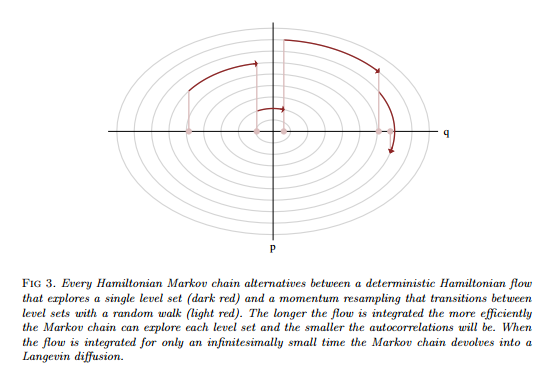
\includegraphics[height=0.5\textheight]{hmc.png}
\end{center}

HMC samples a level set, then deterministically moves along that set.

\vspace{0.3cm}

Long integration time $\implies$ essentially zero autocorrelation in the chain.

\vspace{0.3cm}

(Picture stolen from \url{https://arxiv.org/pdf/1601.00225.pdf})
\end{frame}

\begin{frame}{fragile}
\frametitle{HMC in Practice}
To implement HMC for a differentiable target $\pi(\bm{q})$ you need:
\vspace{0.2cm}
\begin{enumerate}
\item No discrete valued parameters in $\bm{q}$.  
\begin{itemize}
\item Usually can integrate them out, e.g. mixture models.
\end{itemize}
\vspace{0.2cm}
\item No constrained parameters in $\bm{q}$. 
\begin{itemize}
\item Stan: transform and compute the log-Jacobian automatically.
\end{itemize}
\vspace{0.2cm}
\item The gradient vector of $\log \pi(\bm{q})$.
\begin{itemize}
\item Stan: use C++ autodiff library to do this automatically and accurately.
\end{itemize}
\vspace{0.2cm}
\item Choose a kinetic energy, i.e. $\pi(\bm{p}|\bm{q})$.
\begin{itemize}
\item Stan: $\mathrm{N}(\bm{0}, \bm{M})$ and tune $\bm{M}$ during warmup. (Typical HMC)
\item More intelligent: $\bm{M}(\bm{q})$. (Riemannian HMC; future Stan?)
\end{itemize}
\end{enumerate}
\begin{align*}
{\color{red}\Huge{\vdots}}
\end{align*}
\end{frame}

\begin{frame}
\frametitle{HMC in Practice (continued)}
To implement HMC for a differentiable target $\pi(\bm{q})$ you need:
\vspace{0.2cm}
\begin{enumerate}
\item[5.] Numerical integrator for Hamiltonian's equations.
\begin{itemize}
\item Need to make an adjustment to the Hamiltonian flow and use a Metropolis correction to ensure detailed balance.
\vspace{0.2cm}
\item Typically use leapfrog integration $\implies$ how many leapfrog steps ?
\vspace{0.2cm}
\item Stan: adapt number of steps to hit a target Metropolis acceptance rate.
\end{itemize}
\vspace{0.2cm}
\item[6.] An integration time. How long is long enough?
\begin{itemize}
\item Old Stan: No U-Turn Criterion / No U-Turn Sampler (NUTS) \\
\vspace{0.2cm}
``stop when we start heading back toward where we started.''
\vspace{0.2cm}
\item New Stan: eXhaustive HMC (XHMC/XMC/better NUTS) \\
\vspace{0.2cm}
``stop when it looks like autocorrelation should be low.''
\vspace{0.2cm}
\end{itemize}
\end{enumerate}
\end{frame}

\begin{frame}
\frametitle{Why Hamiltonian Monte Carlo?}

The long answer: 
\begin{itemize}
\item \textbf{Everything You \emph{Should} Have Learned About MCMC} \\
(Michael Betancourt) \\
\url{https://www.youtube.com/watch?v=DJ0c7Bm5Djk&feature=youtu.be&t=4h40m10s}
\item \textbf{A Conceptual Introduction to HMC} (Michael Betancourt) \\
\url{https://arxiv.org/pdf/1701.02434.pdf}
\item \textbf{Hamiltonian Monte Carlo for Hierarchical Models} 
(Michael Betancourt and Mark Girolami) \\
\url{https://arxiv.org/pdf/1312.0906.pdf}
\end{itemize}

\vspace{0.5cm}

The short answer: 
\begin{itemize}
\item Works in high dimensions. 
\item More robust. 
\item Makes noise when it fails. 
\end{itemize}

\end{frame}

\begin{frame}
\frametitle{Works in high dimensions}
We are interested in expecations of the form $\int f(\bm{q})\pi(\bm{q})d\bm{q}$.
\begin{itemize}
\item Naively: focus on areas where $f(\bm{q})\pi(\bm{q})$ (density) is large.
\item Better: where where $f(\bm{q})\pi(\bm{q})d\bm{q}$ (mass) is large.
\end{itemize}
\begin{center}
Typical Set:\\
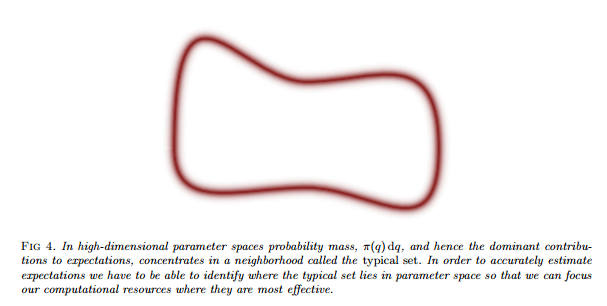
\includegraphics[height=0.4\textheight]{typicalset.png}
\end{center}
In high dimensions, this is essentially a surface.
\begin{itemize}
\item Random walk methods have to take tiny steps.
\item Gibbs methods take a long time to move around the surface.
\item Modes are far away from mass $\to$ mode-based methods fail.
\end{itemize}
\end{frame}

\begin{frame}
\frametitle{Robustness and Noisy Failure}
HMC has guaranteed geometric ergodicity in a larger class of target densities than alternatives.

\vspace{0.5cm}

When geometric ergodicity fails, HMC often won't sample due to numerically infinite gradients.
\begin{center}
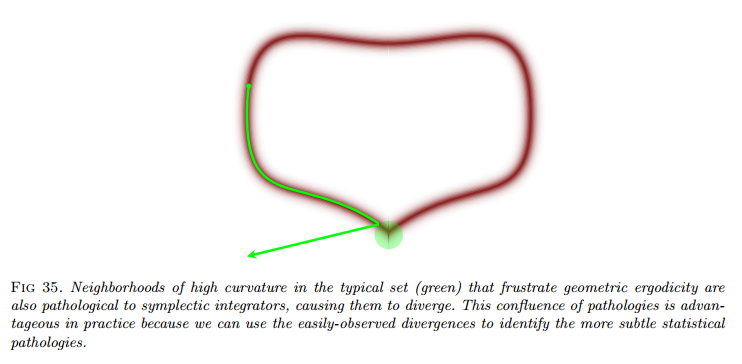
\includegraphics[height = 0.4\textheight]{divergent.png}
\end{center}
\begin{itemize}
\item Caused by weird posterior geometries (reparameterize).
\item Common in hierarchical models.
\item Also a problem in Gibbs samplers, but they still give output.
\end{itemize}
\end{frame}

\begin{frame}[fragile]
\frametitle{Using Stan: Resources}
How to install Stan and \verb0rstan0 (Follow the directions carefully!):
\begin{itemize}
\item \url{https://github.com/stan-dev/rstan/wiki/RStan-Getting-Started}\\~\\
\end{itemize}


Stan manual (it's very good and constantly being improved):
\begin{itemize}
\item \url{https://github.com/stan-dev/stan/releases/download/v2.14.0/stan-reference-2.14.0.pdf} \\~\\
\end{itemize}

Links to the manual, examples, tutorials, and case studies:
\begin{itemize}
\item \url{http://mc-stan.org/documentation/}\\~\\
\end{itemize}

\verb0rstan0 documentation:
\begin{itemize}
\item \url{http://mc-stan.org/interfaces/rstan.html}\\~\\
\end{itemize}

A brief guide to Stan's warnings:
\begin{itemize}
\item \url{http://mc-stan.org/misc/warnings.html}
\end{itemize}
\end{frame}

\begin{frame}[fragile]
\frametitle{Using Stan: A Simple Example}
Define the model in a \verb0.stan0 file:
\begin{verbatim}
data {
  int nobs;
  vector[nobs] y;
}
parameters {
  real mu;
  real<lower = 0> sigma;
}
model {
  y ~ normal(mu, sigma); // mean and sd parameterization
  mu ~ normal(0, 10);
  sigma ~ student_t(5, 0, 10);
}
\end{verbatim}
\end{frame}

\begin{frame}[fragile]
\frametitle{Using Stan: A Simple Example with Hyperparameters}
Or with prior hyperparameters as user inputs: (\verb0normal.stan0)
\begin{verbatim}
data {
  int nobs;
  vector[nobs] y;
  real mu_prior_mn;
  real<lower = 0> mu_prior_sd;
  real<lower = 0> sig_prior_scale;
  real<lower = 0> sig_prior_df;
}
parameters {
  real mu;
  real<lower = 0> sigma;
}
model {
  y ~ normal(mu, sigma); // mean and sd parameterization
  mu ~ normal(mu_prior_mn, mu_prior_sd);
  sigma ~ student_t(sig_prior_df, 0, sig_prior_scale);
}
\end{verbatim}
\end{frame}

\begin{frame}[fragile]
\frametitle{The .stan File}
Defines a target density as a function of data and parameters.
\begin{itemize}
\item Data: all things that are fixed during MCMC, including prior hyperparameters and what we normally think of as ``data''.
\item Parameters: all things we want/need to sample from.\\~\\
\end{itemize}
The file is composed of several ``blocks''. 
\begin{itemize} 
\item ``parameters'' and ``model'' blocks are mandatory. 
\item ``data'' block is necessary to read data into Stan.
\end{itemize}
\begin{verbatim}
data {
  // define all variables to be read into Stan here
}
parameters {
  // define all parameters of the target density here
}
model {
  // define model as a function parameters and data here
}
\end{verbatim}
\end{frame}

\begin{frame}[fragile]
\frametitle{Data Block}
\begin{verbatim}
data {
  int nobs;
  vector[nobs] y;
  real mu_prior_mn;
  real<lower = 0> mu_prior_sd;
  real<lower = 0> sig_prior_scale;
  real<lower = 0> sig_prior_df;
}
\end{verbatim}
\begin{itemize}
\item Must define every single variable that will be read into Stan.
\item Vectors and matrices must have defined dimensions.
\item Can specify bounds for all variables (error checking \& automatic Jacobians).
\item Stan has two basic data types: \verb0int0 and \verb0real0.
\item Vectors and Matrices are collections of \verb0real0s.
\item Can define arrays of \verb0int0s or \verb0real0s... or vectors or whatever.
\item Stan uses \verb0R0 style 1-based indexing.
\item EVERY STATEMENT IN ENDS W/ A SEMICOLON (;)
\item \verb0//0 comments just like \verb0#0 in \verb0R0.
\end{itemize}
\end{frame}

\begin{frame}[fragile]
\frametitle{Some Basic Types}
\begin{verbatim}
real A;                       // scalar real
real<lower = 0> B;            // scalar real > 0
real<upper = 0> C;            // scalar real < 0
real<lower = 0, upper = 1> D; // scalar real > 0 and < 1
vector[10] E;                 // vector of 10 reals
vector<lower = 0>[10] F;      // vector of 10 reals > 0
row_vector[5]         G;      // row vector of 5 reals
F[2]; G[3];                   
matrix[10, 5] H;              // 10x5 matrix of reals
H[1,3]; H[6];                 // H[6] = 6th row of H
// special functions for accessing columns or slices of H
cov_matrix I[2];              // 2x2 PD matrix
corr_matrix J[2];             // 2x2 PD matrix
cholesky_factor_cov K[2];     // lower triangular
cholesky_factor_corr L[2];    // lower triangular
simplex M[5];  
// many more
\end{verbatim}
\end{frame}

\begin{frame}[fragile]
\frametitle{Transformed data and parameters}
Transformed data: once before running MCMC.\\
Transformed parameters: once per leapfrog step.\\
\begin{verbatim}
data { ... }
transformed data {
  vector[n_obs] log_y;
  log_y = log(y);
}
parameters = { 
  real<lower = 0> sigma2; ...
}
transformed parameters {
  real<lower = 0> sigma;
  sigma = sqrt(sigma);
}
model { 
  log_y ~ normal(mu, sigma)
  sigma2 ~ inv_gamma(.,.); ...
}
\end{verbatim}
\end{frame}

\begin{frame}[fragile]
\frametitle{Transformations in the model block}
Useful for intermediate quantities you don't want MCMC draws for.\\
No constraints allowed here.
\begin{verbatim}
model {
  real sigma;
  sigma = sqrt(sigma2);
  log_y ~ normal(mu, sigma)
  sigma2 ~ inv_gamma(.,.); ...
}
\end{verbatim}
\end{frame}
\end{document}
